% !TEX root = epifanov_solid_state_physics.tex
%!TEX TS-program = pdflatex
%!TEX encoding = UTF-8 Unicode


\chapter[Magnetic Properties of Solids]{Magnetic Properties of Solids}\label{chap:7}
% \chaptermark{The Band Theory of Solids}

\section{Magnetic field in magnetic materials}\label{sec:63}

Let us place a homogeneous body of volume $V$ into a uniform magnetic field of intensity $\vec{H}$ and induction $\vec{B}_0=\mu_0\vec{H}$. Acted upon by the field, the body becomes magnetized obtaining a magnetic moment $M$. The ratio of the magnetic moment to the volume of the body is termed \textit{magnetization}, $\ab{J}{m}$:
\begin{equation}\label{eq:7_1}
    \ab{J}{m} = \frac{M}{V},
\end{equation}

\noindent
and when magnetization is not uniform it is equal to
\begin{equation}\label{eq:7_2}
    \ab{J}{m} = \diff{M}{V}.
\end{equation}

Magnetization is a vector; in uniform magnetic, bodies $\ab{J}{m}$ is either directed parallel or antiparallel to $\vec{H}$. The unit of magnetic moment in the SI system is \si{\ampere\metre\squared} and that of magnetization is \si{\ampere\per\metre}.

The ratio of magnetization $\ab{J}{m}$ to the magnetic field intensity $H$ is termed the \textit{magnetic susceptibility}, $\chi$:
\begin{equation}\label{eq:7_3}
    \chi = \frac{\ab{J}{m}}{H}.
\end{equation}

\noindent
It may easily be seen that $\chi$ is a dimensionless quantity. From \eqn{7_3}, we get
\begin{equation}\label{eq:7_4}
    \ab{J}{m} = \chi H.
\end{equation}

A magnetized body placed in an external field, establishes its own field which in isotropic magnetic materials, away from its external boundaries, is directed either parallel or antiparallel to the external field. Denote the external field induction by $B_0$, the proper field induction by $B_1$ and the resultant induction by $B$. For uniform magnetic materials, $B$ is an algebraic sum of $B_0$ and $B_1$:
\begin{equation}\label{eq:7_5}
    B = B_0 + B_1.
\end{equation}

\noindent
Experiments show that
\begin{equation}\label{eq:7_6}
    B_1 = \mu_0 \ab{J}{m} = \chi B_0
\end{equation}

\noindent
wherefore
\begin{equation}\label{eq:7_7}
    B = (1 + \chi) B_0.
\end{equation}

\noindent
The quantity
\begin{equation}\label{eq:7_8}
    \mu = 1 + \chi
\end{equation}

\noindent
is termed \textit{magnetic permeability}. It follows from \eqn{7_8} that
\begin{equation}\label{eq:7_9}
    \chi = \mu - 1.
\end{equation}

\noindent
Substituting \eqn{7_8} into \eqref{eq:7_7}, we obtain
\begin{equation}\label{eq:7_10}
    B = \mu B_0 = \mu \mu_0 H.
\end{equation}

\noindent
The unit of field intensity $H$ in the SI system is \si{\ampere\per\metre} and that of induction $B$ the tesla (\si{\tesla}).

\section{Magnetic properties of solids}\label{sec:64}

All materials may be divided into three large groups according to the absolute value and the sign of their magnetic susceptibility (\tab{7_1}): diamagnetics, paramagnetics and ferromagnetics.

\begin{table}[!b]
	\renewcommand{\arraystretch}{1.2}
	\caption{}
	\vspace{-0.6cm}
	\label{table:7_1}
	\begin{center}\resizebox{0.98\linewidth}{!}{
			\begin{tabular}{lclclc}
				\toprule[1pt]
                \multicolumn{2}{c}{\textbf{Diamagnetics}} & \multicolumn{2}{c}{\textbf{Paramagnetics}} & \multicolumn{2}{c}{\textbf{Ferromagnetics}}\\
                \cline{1-2}\cline{3-4}\cline{5-6}
                \textbf{Substance} & $\chi=\mu-1$ & \textbf{Substance} & $\chi=\mu-1$ & \textbf{Substance} & $\chi=\mu-1$\\
                \midrule[0.5pt]\midrule[0.5pt]
                \ce{Bi} & \num{-18e-5} & \ce{CaO} & \num{580e-5} & \ce{Fe} & \num{1000}\\
                \ce{Cu} & \num{-0.9e-5} & $\ce{FeCl2}$ & \num{360e-5} & \ce{Co} & \num{240}\\
                \ce{Ge} & \num{-0.8e-5} & $\ce{NiSO4}$ & \num{120e-5} & \ce{Ni} & \num{150}\\
                \ce{Si} & \num{-0.3e-5} & \ce{Pt} & \num{26e-5} & & \\
				\bottomrule[1pt]
			\end{tabular}
	}\end{center}
\end{table}

\textbf{Diamagnetics and paramagnetics.} For diamagnetics ($|\chi|<1$), $\chi$ is negative and independent of the intensity of the external magnetic field and of temperature. Such materials are magnetized in the direction opposite to the direction of the external field and because of that they are pushed out of the regions of the highest field intensity.

Paramagnetics also have $|\chi|<1$, but contrary to diamagnetics $\chi$ is positive. Such bodies are magnetized in the direction of the external field and are drawn into the regions of maximum $H$.

Figure \ref{fig:7_1}(a) shows the dependence of $\ab{J}{m}$ on the field intensity for diamagnetics, $1$, and for paramagnetics, $2$. In both cases $\ab{J}{m}$ is proportional to $H$, this being an indication of the independence of $\chi$ of $H$. However, for paramagnetics this is observed only in relatively weak fields at high temperatures; in strong fields and at low temperatures the plot $\ab{J}{m}(H)$ asymptotically approaches the limit value $\ab{J}{s}$, which corresponds to magnetic ``saturation'' of the paramagnetic [\fig{7_1}(b)]. Besides, $\chi$ of paramagnetic bodies is dependent on temperature. This dependence was first studied by Pierre Curie. He demonstrated that
\begin{equation}\label{eq:7_11}
    \chi = \frac{C}{T}
\end{equation}

\noindent
where $T$ is the absolute temperature of the paramagnetic, and $C$ is a constant dependent on its nature. The term for it is the \textit{Curie constant} and for expression \eqref{eq:7_11} the \textit{Curie law}.

\begin{figure}[t]
	\begin{center}
		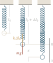
\includegraphics[scale=1]{figures/ch_07/fig_7_1.pdf}
		\caption[]{Magnetization $\ab{J}{m}$ versus the magnetic field intensity $H$: (a)---diamagnetics ($1$) and paramagnetics ($2$) in weak and medium fields at normal and high temperatures; (b)---paramagnetics at low temperatures (or in very strong fields).}
		\label{fig:7_1}
	\end{center}
	\vspace{-0.7cm}
\end{figure}

\textbf{Ferromagnetics.} Magnetic susceptibility $\chi$ of ferromagnetic materials, a typical representative of which is iron, is also positive but immeasurably greater than that of paramagnetics. Besides, $\chi$ depends on $H$. Apart from iron this group includes also nickel, cobalt, gadolinium, dysprosium, holmium, erbium and some alloys.

The rules governing the magnetization were first investigated by the Russian physicist A. G. Stoletov. Figure \ref{fig:7_2} shows the dependence
of $B$ (a), of magnetization $\ab{J}{m}$ (b), and of susceptibility $\chi$ (c) on $H$ for soft iron. $B$ and $\ab{J}{m}$ at first rise quickly with the magnetizing field but then the rise slows down and, at some $\ab{H}{s}$, a close to the maximum value of $\ab{J}{s}$ is attained; any further slow increase
in induction is due solely to the increase in $H$. This state corresponds to technical saturation of the ferromagnetic: as this state is approached, $\chi\to 0$.

\begin{figure}[t]
	\begin{center}
		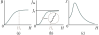
\includegraphics[scale=1]{figures/ch_07/fig_7_2.pdf}
		\caption[]{Magnetization of ferromagnetics: (a)---induction $B$ versus field intensity $H$; (b)---magnetization $\ab{J}{m}$ versus field intensity $H$ (the right-hand side shows a magnified section of the magnetization curve); (c)---magnetic susceptibility versus field intensity $H$.}
		\label{fig:7_2}
	\end{center}
	\vspace{-0.7cm}
\end{figure}

A careful study of the magnetization curve shows that as $H$ increases $\ab{J}{m}$ rises not continuously but stepwise. This is especially apparent in the region of the steep rise of the magnetization curve. Figure \ref{fig:7_2}(b) shows a magnified section of the magnetization curve (enclosed in a circle). This section consists of a large number of steps corresponding to individual jumps accompanying the variation of $\ab{J}{m}$ with a continuous rise in $H$. The stepwise nature of the magnetization process was discovered by Heinrich Barkhausen and became known as the \textit{Barkhausen effect}.

Figure \ref{fig:7_3} shows the plot of a complete remagnetizing cycle of a ferromagnetic. It may be seen from \fig{7_3} that during the remagnetization, the variation of $B$ lags behind the variation of $H$, and when $H=0$ is not equal to zero but to $\ab{B}{res}$. This lagging of $B$ behind $H$ has been named \textit{magnetic hysteresis} and the induction $\ab{B}{res}$ \textit{residual magnetic induction}, or \textit{remanence}.
To remove it, a demagnetizing field $\ab{H}{c}$ termed \textit{coersive force} should be applied. The closed curve A$\ab{B}{res}\ab{H}{c}$A$'\ab{B}{res}'\ab{H}{c}'$A, which describes the remagnetizing cycle, is termed the hysteresis loop. The area of this loop is proportional to the work that should be expended to remagnetize a ferromagnetic of unit volume. In the course of remagnetization, this work is completely
transformed into heat. Therefore, when the ferromagnetic is remagnetized many times in succession its temperature rises, the effect being the greater the greater the area of the hysteresis loop.

\begin{figure}[t]
	\begin{center}
		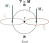
\includegraphics[scale=1]{figures/ch_07/fig_7_3.pdf}
		\caption[]{Hysteresis loop.}
		\label{fig:7_3}
	\end{center}
	\vspace{-0.7cm}
\end{figure}

Ferromagnetic materials are classified as ``soft'' and ``hard'', or having a high coersive force. Soft magnetic materials used for manufacturing cores of electric motors and instruments have a low coersive force and high permeability. The best alloys of this type (Supermalloy, for instance) have $\mu$'s as high as \num{e6}, saturation induction $\ab{B}{s}\approx\SI{1}{\tesla}$ and a coersive force $\ab{H}{c}$ of only \SI{0.32}{\ampere\per\metre}. Their hysteresis-
loop area is so small that their remagnetization losses are some $500$ times less than those of soft iron. Hard magnetic materials are characterized by a high coersive force and by high residual magnetization. For instance, Magnico, used for manufacturing permanent magnets, has $\ab{H}{c}\approx\SI{5e5}{\ampere\per\metre}$ and $\ab{B}{res}=\SI{1.35}{\tesla}$.

When ferromagnetic materials are heated, their magnetic properties become less pronounced: there is a drop in the values of $\chi$, $\mu$, $\ab{J}{m}$, etc. There is a temperature $\ab{\Theta}{C}$ for every ferromagnetic at which it looses its ferromagnetic properties. This is known as the \textit{ferromagnetic Curie point}. By way of an example we shall show the Curie points of some ferromagnetics: cobalt, \SI{1150}{\degreeCelsius}; iron, \SI{770}{\degreeCelsius}; Nickel, \SI{360}{\degreeCelsius}; $30\%$ permalloy, \SI{70}{\degreeCelsius}.

Above $\ab{\Theta}{C}$, ferromagnetics turn into paramagnetics with their characteristic linear dependence of $1/\chi$ on $T$ (\fig{7_4}), which is quite well represented by the following relation, known as the \textit{Curie-Weiss law}:
\begin{equation}\label{eq:7_12}
    \chi = \frac{C}{T - \Theta}
\end{equation}

\noindent
with $C$ the Curie constant and $\Theta$ the \textit{paramagnetic Curie point} (it is somewhat higher than $\ab{\Theta}{C}$).

\begin{figure}[!t]
	\begin{minipage}[t]{0.48\linewidth}
		\begin{center}
			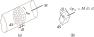
\includegraphics[scale=1]{figures/ch_07/fig_7_4.pdf}
			\caption[]{Temperature dependence of magnetic susceptibility of ferromagnetics: $\ab{\Theta}{C}$ the ferromagnetic Curie point; and $\Theta$ the paramagnetic Curie point.}
			\label{fig:7_4}
		\end{center}
	\end{minipage}
	\hfill{ }%\hspace{-0.1cm}
	\begin{minipage}[t]{0.48\linewidth}
		\begin{center}
			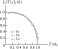
\includegraphics[scale=1]{figures/ch_07/fig_7_5.pdf}
			\caption[]{Temperature dependence of maximum magnetization of iron, nickel and cobalt.}
			\label{fig:7_5}
		\end{center}
	\end{minipage}
\vspace{-0.3cm}
\end{figure}

Figure \ref{fig:7_5} shows the temperature dependence of maximum magnetization of iron, nickel, and cobalt. The ratio $T/\ab{\Theta}{C}$ is plotted along the $x$ axis and the ratio $\ab{J}{s}(T)/\ab{J}{s}(0)$ along the $y$ axis. In such relative coordinates the dependence of magnetization on temperature is described by the same curve for all ferromagnetics. As temperature rises, magnetization drops becoming practically zero at the Curie point.

\begin{figure}[t]
	\begin{center}
		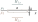
\includegraphics[scale=1]{figures/ch_07/fig_7_6.pdf}
		\caption[]{Magnetization plots of iron (a) and nickel (b) single crystals in directions $[100]$, $[110]$ and $[111]$.}
		\label{fig:7_6}
	\end{center}
	\vspace{-0.7cm}
\end{figure}

Ferromagnetic single crystals are characterized by anisotropic magnetization. Figure \ref{fig:7_6} shows the magnetization curves of iron (a) and nickel (b) crystals in the $[111]$, $[110]$, and $[100]$ directions. It follows from \fig{7_6}, that there are directions in the single crystal, in which it is easier to magnetize the crystal and obtain magnetic saturation at relatively small values of magnetic field intensity. Those directions are termed \textit{directions of easy magnetization}. For iron this direction is the $[100]$, and for nickel the
$[111]$ direction. It is much more difficult to magnetize iron in the $[110]$ and $[111]$ directions, and nickel in the $[110]$ and $[100]$ directions, substantially greater values of magnetic field intensity being needed to attain magnetic saturation. Those directions are termed \textit{difficult magnetization directions}. The integral
\begin{equation}\label{eq:7_13}
    \ab{W}{m} = \int_0^{\ab{J}{s}} \mu_0 H \, \deriv{\ab{J}{m}}
\end{equation}

\noindent
taken along the magnetization curve expresses the work spent on magnetizing the crystal in the given direction. This work is transformed into free energy of the magnetized crystal. It may be seen from \fig{7_6}, that the least free energy is that of the crystal magnetized in the easy direction and the greatest is that of the crystal magnetized in the difficult direction.

Magnetization of ferromagnetics is accompanied by a change in their dimensions and shape. This phenomenon became known as \textit{magnetostriction}. Figure \ref{fig:7_7} shows the relative change in the length of rods made of nickel, of annealed and of cast cobalt, of iron, and of steel magnetized in fields of gradually increasing intensity. The greatest relative contraction is that of nickel (almost $0.004$ percent); iron and steel rods increase their length a little in weak fields and contract in strong fields. On the contrary, cast cobalt rods contract in weak fields and increase their length in strong fields.

In compliance with the Le Chatelier principle to the effect that a system resists the influence of external factors striving to change its state, the mechanical deformation of ferromagnetic bodies resulting in the change in their shape and dimensions should influence the magnetization of such bodies. Specifically, if the body being magnetized contracts in the given direction, then application of a compressive stress in this direction should favour magnetization and application of an extending stress should make magnetization more difficult. The variation of magnetic properties of strained ferromagnetic bodies is termed the \textit{magnetoelastic effect}. Some ferromagnetic materials are so sensitive to internal stresses caused by deformations that this property is utilized for the purposes of strain measurements.

\begin{figure}[t]
	\begin{center}
		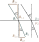
\includegraphics[scale=1]{figures/ch_07/fig_7_7.pdf}
		\caption[]{Variation of length of ferromagnetic samples with magnetization (magnetostriction).}
		\label{fig:7_7}
	\end{center}
	\vspace{-0.7cm}
\end{figure}

When a ferromagnetic is magnetized in an alternating magnetic field, its dimensions change with a frequency double that of the field. This property is used in \textit{magnetostrictive oscillator} capable of generating powerful ultrasonic vibrations with a frequency up to several megahertz. Such oscillators are employed in ultrasonic devices for the machining and cleaning of solid objects, in sonars used to measure depth of waterways, and in numerous other devices and instruments.

\begin{figure}[t]
	\begin{center}
		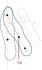
\includegraphics[scale=1]{figures/ch_07/fig_7_8.pdf}
		\caption[]{Dependence of linear expansion coefficient of iron-nickel (a) and of iron-platinum (b) alloys on composition.}
		\label{fig:7_8}
	\end{center}
	\vspace{-0.7cm}
\end{figure}

An interesting problem is that of thermal expansion of ferromagnetic bodies. Thermal expansion of solids is, as we know, due to the anharmonicity of vibrations of particles around their equilibrium sites. For diamagnetic and paramagnetic solids, anharmonicity is the only cause of the change in their dimensions upon heating. By force of this such bodies always expand with the rise in temperature. Let us denote the linear expansion coefficient due to anharmonicity of atomic vibrations by $\alpha_1$. The situation in ferromagnetic materials is not so simple. A change in their temperature is accompanied by a change in their magnetization and, consequently, in dimensions. N. S. Akulov has proposed the term \textit{thermostriction} for this phenomenon. Denote the linear expansion coefficient due to thermostriction by $\alpha_2$. The total thermal expansion coefficient of a ferromagnetic will be $\alpha=\alpha_1+\alpha_2$. The coefficient $\alpha_1$ is always positive while $\alpha_2$ may be either positive or negative. Therefore, the total thermal expansion coefficient of a ferromagnetic material may be positive, zero, or negative. For instance, the group of ferromagnetic materials with a negative ``ferromagnetic'' component of the thermal linear expansion coefficient includes Invar alloys. Figure \ref{fig:7_8} shows the dependence of the thermal expansion coefficient of iron-nickel (a) and iron-platinum (b) alloys on their composition. The $\alpha$ of alloys containing about $36\%$ nickel is about $10$ times less than that of pure nickel or iron: $\alpha$ of alloy containing $56\%$ platinum is negative, such an alloy does not expand upon heating but, on the contrary, contracts.

Invar alloys are widely used in instrument manufacture, metrology, aviation, and manufacture of electric lamps and radio valves. Depending on practical purposes, alloys with very small, zero, or even negative thermal expansion coefficients can be used.

\section{Magnetic properties of atoms}\label{sec:65}

\begin{figure}[t]
	\begin{center}
		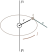
\includegraphics[scale=1]{figures/ch_07/fig_7_9.pdf}
		\caption[]{Orbital magnetic moment $\mu_l$, and orbital angular momentum $p_l$ of an electron.}
		\label{fig:7_9}
	\end{center}
	\vspace{-0.7cm}
\end{figure}

\textbf{The orbital magnetic moment of an atom.} The atom of every element is made up of a positively charged nucleus and an electron shell. Many magnetic phenomena can be adequately explained with the aid of Bohr's theory, in which it is assumed that the electrons of the shell move in definite orbits. Each such electron will establish a closed current equal to $I=-q\nu$ ($\nu$ is the frequency of rotation of the electron in the orbit, and $q$ its charge). The magnetic moment of the current is $M=IS=-q\nu S$ ($S$ is the area of the orbit). Since $S=\pi r^2$ and $\nu=v/(2\pi r)$ ($v$ is the linear velocity of the electron in the orbit), it follows that
\begin{equation}\label{eq:7_14}
    M = \mu_l = - \frac{vqr}{2}.
\end{equation}

The magnetic moment of the electron, which is due to its motion around the nucleus, is termed \textit{orbital magnetic moment}. We shall denote it by $\mu_l$. This moment is perpendicular to the plane of the orbit as is required by the right-hand screw rule (\fig{7_9}).

The orbital angular momentum of the electron is
\begin{equation}\label{eq:7_15}
    p_l = mvr
\end{equation}

\noindent
where $m$ is the electron mass. It is opposite to $\mu_l$. Comparing Eqs. \eqref{eq:7_14} and \eqref{eq:7_15}, we find
\begin{equation}\label{eq:7_16}
    \mu_l = - \frac{q}{2m} p_l.
\end{equation}

\noindent
The ratio
\begin{equation}\label{eq:7_17}
    \gamma_l = \frac{\mu_l}{p_l} = - \frac{q}{2m}
\end{equation}

\noindent
is termed the \textit{gyromagnetic ratio}.

As required by quantum mechanics, $\vec{p}_l$ and its projection $p_{lH}$ on the direction of the magnetic field $H$, can assume only discrete values, namely
\begin{align}
    p_l &= \hslash [l (l + 1)]^{1/2}, \label{eq:7_18}\\
    p_{lH} &= m_l \hslash \label{eq:7_19},
\end{align}

\noindent
where $l$ is the orbital quantum number, which can assume only the following values:
\begin{equation}\label{eq:7_18p}
    l = 0, 1, 2, \ldots, n \tag{7.18$'$}
\end{equation}

\noindent
$n$ values in all ($n$ is the principal quantum number); $m_l$ is the magnetic quantum number, which can assume only the following values:
\begin{equation}\label{eq:7_19p}
    m_l = -l, -(l-1), \ldots, 0, \ldots, +l \tag{7.19$'$}
\end{equation}

\noindent
$2l+1$ values in all.

Because of that, the magnetic moment $\mu_l$ and its projection $\mu_{lH}$ on the direction of $H$ may assume only the following discrete values:
\begin{align}
    \mu_l &= - \frac{q\hslash}{2m} [l (l + 1)]^{1/2} = -\ab{\mu}{B} [l (l + 1)]^{1/2}, \label{eq:7_20}\\
    \mu_{lH} &= - m_l \ab{\mu}{B} \label{eq:7_21},
\end{align}

\noindent
where
\begin{equation}\label{eq:7_22}
    \ab{\mu}{B} = - \frac{q\hslash}{2m} = \SI{9.27e-24}{\ampere\metre\squared}
\end{equation}

\noindent
is the \textit{Bohr magneton}. It is the ``quantum'' of the magnetic moment and is accepted as a unit for measuring magnetic moments of atomic systems.

In a complex atom whose electron shell is made up of many electrons, the total orbital magnetic moment is found by adding up the moments of individual electrons in compliance with the rules of space quantization. The moment of closed electron shells is zero. By force of this only, the atoms with partially filled shells can have a nonzero orbital magnetic moment. But even in the latter case, should the partially filled shell lie close to the external shell and should the interaction of the atoms in the solid state be strong, the magnetic moments of the partially filled shell would be ``frozen in'': their orientation in an external field would be so impaired that they would take practically no part in the magnetization of the body. For instance, such is the behaviour of orbital magnetic moments of the electrons of the partially filled \enlevel{3}{d}{} shell of the elements belonging to the iron group.

\textbf{The spin magnetic moment of an atom.} Apart from the orbital angular momentum, the electron has an intrinsic angular momentum $p_s$ termed \textit{spin}. It is known from quantum mechanics that
\begin{equation}\label{eq:7_23}
    p_s = \sqrt{3} \frac{\hslash}{2}
\end{equation}

\noindent
and that the projection of the spin on the direction of the field $H$ may assume only the following values:
\begin{equation}\label{eq:7_24}
    p_{sH} = \pm \frac{\hslash}{2}.
\end{equation}

There is an intrinsic magnetic moment $\mu_s$ connected with the intrinsic electron angular momentum whose value was first experimentally determined by Otto Stern and Walther Gerlach. Their experiments demonstrated that the projection $\mu_{sH}$ is numerically equal to the Bohr magneton:
\begin{equation}\label{eq:7_25}
    \mu_{sH} = \pm \ab{\mu}{B} = \pm \frac{q\hslash}{2m} = - \frac{q}{m} p_{sH}
\end{equation}

\noindent
(the minus sign reflects the negative nature of the electron charge). The gyromagnetic ratio for the intrinsic moments of the electron is
\begin{equation}\label{eq:7_26}
    \gamma_s = \frac{\mu_{sH}}{p_{sH}} = - \frac{q}{m}.
\end{equation}

\noindent
It is twice as large as $\gamma_l$ for the orbital moments.

In atoms containing a large number of electrons, $p_s$ should be added up like vectors with account taken of the rules of space quantization. The total spin moment of closed shells is zero, the same as the orbital moment. Table \ref{table:7_2} shows, by way of an example, the data on the spin configuration of the \enlevel{3}{d}{} shell of free atoms of the elements of the iron group.

\begin{table}[!b]
	\renewcommand{\arraystretch}{1.2}
	\caption{}
	\vspace{-0.6cm}
	\label{table:7_2}
	\begin{center}\resizebox{0.98\linewidth}{!}{
			\begin{tabular}{lcccccccc}
				\toprule[1pt]
                & Sc & Ti & V & Cr & Mn & Fe & Co & Ni\\
                \midrule[0.5pt]\midrule[0.5pt]
                \multirow{2}{*}{Total spin} & $1$ & $2$ & $3$ & $5$ & $5$ & $4$ & $3$ & $2$\\
                & $\downarrow$ & $\downarrow\downarrow$ & $\downarrow\downarrow\downarrow$ & $\downarrow\downarrow\downarrow\downarrow\downarrow$ & $\downarrow\downarrow\downarrow\downarrow\downarrow$ & $\downarrow\uparrow\downarrow\downarrow\downarrow\downarrow$ & $\downarrow\uparrow\downarrow\uparrow\downarrow\downarrow\downarrow$ & $\downarrow\uparrow\downarrow\uparrow\downarrow\uparrow\downarrow\downarrow$\\
				\bottomrule[1pt]
			\end{tabular}
	}\end{center}
\end{table}

The spins are least compensated in the chromium and manganese atoms and, correspondingly, they have the maximum total spin moment. However, such orientation of the spins is not usually retained in the solid state and, because of that, the total atomic spin moment in the solid is different. For instance, in the iron lattice, the average number of Bohr magnetons per atom is not $4$ but only $2.3$; in chromium it is $0.4$, and in \ce{\alpha}-manganese it is $0.5$.

\textbf{Magnetic moments of nucleus.} Atomic nuclei too have a spin and a magnetic moment connected with it. The order of magnitude of the nuclear spin is the same as that of the electron. Since the nuclear mass is some \num{e3} times greater than the electron mass, the nuclear magnetic moment, in compliance with \eqn{7_25}, is three orders of magnitude less than the electron magnetic moment. Therefore, as a first approximation, the effect of nuclear magnetic moments on the magnetic properties of bodies can be neglected. This does not mean that those moments do not play any role at all. In some phenomena, not discussed in this book, that role may be quite important.

\textbf{The total magnetic moment of an atom.} The total magnetic moment of the electron shell of the atom is determined as follows. Using the rules of space quantization, one finds the total orbital angular momentum: $P_L=\sum_i p_{li}$, where $p_{li}$ is the orbital angular momentum of the $i$-th electron. The numerical value of $P_L$ is determined by the quantum number $L$
\begin{equation}\label{eq:7_27}
    P_L = \hslash [L (L + 1)]^{1/2}.
\end{equation}

\noindent
The number $L$ may be any integer between the maximum and the minimum values of the algebraic sum $\sum_i l_i$ of the orbital quantum numbers $l_i$ of individual electrons. Next, one finds the total atomic spin: $P_S=\sum_i p_{si}$, where $p_{si}$ is the spin of the $i$-th electron. The numerical value of $P_S$ is determined by the quantum number $S$:
\begin{equation}\label{eq:7_28}
    P_S = \hslash [S (S + 1)]^{1/2}.
\end{equation}

\noindent
The number $S$ may assume values lying in the interval between the maximum and the minimum values of the algebraic sum $\sum_i s_i$ of spin quantum numbers of the individual electrons, the difference between successive values of $S$ being unity.

Finally, one finds the total atomic momentum $\vec{P}_J$, equal to the vector sum of $\vec{P}_L$ and $\vec{P}_S$, that is $\vec{P}_J=\vec{P}_L+\vec{P}_S$. The numerical value of $\vec{P}_J$ is determined by the intrinsic quantum number $J$:
\begin{equation}\label{eq:7_29}
    P_J = \hslash [J (J + 1)]^{1/2}.
\end{equation}

\noindent
which may assume the following set of values:
\begin{equation}\label{eq:7_30}
    \begin{split}
        J &= L+S, L+S-1, \ldots, L-S, \quad\text{if}\quad L>S\\
        J &= S+L, S+L-1, \ldots, S-L, \quad\text{if}\quad S>L.
    \end{split}
\end{equation}

\noindent
The only allowed orientations of $\vec{P}_J$ in an external field are such that its projections on the direction of the field are multiples of $\hslash$:
\begin{equation}\label{eq:7_31}
    P_{JH} = m_J \hslash,
\end{equation}

\noindent
where $m_J$ is the magnetic quantum number equal to
\begin{equation}\label{eq:7_32}
    m_J = -J, -(J-1), \ldots, 0, 1, 2, \ldots, J
\end{equation}

\noindent
$2J+1$ values in all.

The atomic magnetic moment corresponding to the total momentum $P_J$ is
\begin{equation}\label{eq:7_33}
    M_J = - g \ab{\mu}{B} [J (J + 1)]^{1/2}
\end{equation}

\noindent
with projections on the direction of an external field $H$ equal to
\begin{equation}\label{eq:7_34}
    M_{JH} = - m_J g \ab{\mu}{B}
\end{equation}

\noindent
where
\begin{equation}\label{eq:7_35}
    g = 1 + \frac{J(J+1) + S(S+1) - L(L+1)}{2J(J+1)}
\end{equation}

\noindent
is the \textit{Lande factor} or \textit{magnetic splitting factor}, which takes account of the difference in gyromagnetic ratios of the orbital and the spin moments making up the total atomic magnetic moment. For $L=0$, that is, in the case of a purely spin magnetism, $g=2$; for $S=0$, that is, in the case of a purely orbital magnetism, $g=1$.

Often the term atomic magnetic moment is taken to mean not \eqn{7_33}, but the maximum value of the projection $M_{JH}$. For instance, the magnetic moment of a hydrogen atom in the ground state ($L=0, S=1/2, g=2$) characterized by $J=1/2$ is taken to be equal to $\ab{\mu}{B}$; for a free iron atom with a ``frozen in'' orbital magnetic moment, $J=S=2$, $g=2$ and $\ab{M}{a}= 4\ab{\mu}{B}$.

All atoms and ions with closed shells have $S=0$, $L=0$, and $J=0$. Therefore, the magnetic moments of such atoms and ions are zero. Paramagnetism owes its existence to the presence in an atom of partially filled shells. According to the Pauli exclusion principle, there may not be more than two electrons with opposite spins in one state. The total spin moment of those electrons is zero. Such electrons are termed \textit{paired}. If an atom or an ion contains an odd number of electrons, one of them will be unpaired and the atom will have a permanent magnetic moment. If the atom contains an even number
of electrons, two cases are possible: either all electrons are paired and the total spin moment is zero or two or more electrons are unpaired and the atom has a permanent magnetic moment. For instance, H, K, Na, Ag have odd numbers of electrons, one of them unpaired; Be, C, He, Mg contain even numbers of electrons, all of them paired. Oxygen also contains an even number of electrons, but two of them are unpaired.

Magnetic moments of many molecules are zero because only some of them contain unpaired electrons. First of all, these are the free radicals, which play an exceptionally important part in many chemical reactions. As examples of such, radicals are free hydroxyl (OH), free methyl ($\ce{CH3}$), and free ethyl ($\ce{C2H5}$). The presence of unpaired electrons in molecules and in free radicals makes them magnetic.

\textbf{Classification of magnetic materials.} When the orbital and the spin moments are added up, a complete compensation may take place and then the total atomic moment will be zero. If such a compensation does not take place, the atom will have a permanent magnetic moment. Accordingly, the magnetic properties of bodies will be different.

\begin{figure}[t]
	\begin{center}
		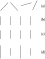
\includegraphics[scale=1]{figures/ch_07/fig_7_10.pdf}
		\caption[]{Schematic representation of atomic magnetic moments in paramagnetic (a), ferromagnetic (b), antiferromagnetic (c), and ferrimagnetic (d) materials.}
		\label{fig:7_10}
	\end{center}
	\vspace{-0.7cm}
\end{figure}

Materials whose atoms have no permanent magnetic moments are diamagnetic. Materials whose atoms have a permanent magnetic moment may be either paramagnetic, ferromagnetic, antiferromagnetic,
or ferrimagnetic. Namely, if the interaction between the atomic magnetic moments is zero or very weak, the material will be paramagnetic [\fig{7_10}(a)]; if the neighbouring magnetic moments tend to align themselves parallel to one another, the material will
be ferromagnetic [\fig{7_10}(b)]; if the neighbouring magnetic moments tend to align themselves antiparallel to one another, the material will be antiferromagnetic [\fig{7_10}(c)]; finally, if the neighbouring magnetic moments tend to align themselves antiparallel to one another but their magnitude is not the same, then the material will be ferrimagnetic [\fig{7_10}(d)].

\section{Origin of diamagnetism}\label{sec:66}

The cause of diamagnetism is a change in the orbital motion of the electrons acted upon by an external magnetic air field. It is common to materials but is often overshadowed by strong para- and ferromagnetism. In its pure form, diamagnetism is displayed by materials whose total atomic magnetic moment is zero.

\begin{figure}[t]
	\begin{center}
		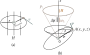
\includegraphics[scale=1]{figures/ch_07/fig_7_11.pdf}
		\caption[]{Effect of magnetic field on orbital motion of an electron: (a)---field $H$ is perpendicular to orbit plane; (b)---orbit precession in magnetic field.}
		\label{fig:7_11}
	\end{center}
	\vspace{-0.7cm}
\end{figure}

\textbf{Precession of electron ``orbits'' in a magnetic field.} Consider the motion of an electron in an orbit of radius $r$ [\fig{7_11}(a)]. In the
absence of field $H$, the centripetal force applied to the electron is $\ab{F}{cp}=mv_0^2/r=m\omega_0^2r$ ($v_0$ is the linear and $\omega_0$ the angular velocity of the electron's motion). When external field $H$, perpendicular to the plane of the orbit is applied, the electron is acted upon by the Lorentz force $\ab{F}{L}=qv_0B_0$ directed along the radius of the orbit ($B_0$ is the field's induction). The resultant centripetal force will be
\begin{equation*}
    F = \ab{F}{cp} + \ab{F}{Lorentz} \quad\text{or}\quad m \omega^2 r = m \omega_0^2 r + q \omega_0 r B_0.
\end{equation*}

\noindent
It follows that
\begin{equation}\label{eq:7_36}
    mr (\omega^2 - \omega_0^2) = mr (\omega - \omega_0) (\omega + \omega_0) \approx 2 m r \omega_0 \ab{\omega}{L} = q \omega_0 B_0
\end{equation}

\noindent
where
\begin{equation}\label{eq:7_37}
    \ab{\omega}{L} = \omega - \omega_0 = \frac{q}{2m} B_0 = \frac{q}{2m} \mu_0 H
\end{equation}

\noindent
is called the \textit{Larmor angular frequency}.

Thus, a magnetic field changes the angular frequency of an orbiting electron. It may be seen from \eqn{7_37} that this change is the same for all electrons no matter what the radius of their orbits and the linear velocity of their motion are. The direction of $\ab{\omega}{L}$ coincides with that of $B_0$.

Generally, when $H$ is not perpendicular to the plane of the orbit, its effect is to excite precession of the orbit around the direction of
the field [\fig{7_11}(b)]: the perpendicular $\vec{p}_l$ to the plane of the orbit describes a cone around $H$. Calculations show that the angular
velocity of such a precession is expressed by \eqn{7_37}.

\textbf{Induced magnetic moment of an atom. Magnetic susceptibility of diamagnetics.} The precession of the electron orbit results in an additional motion of the electron around field $H$. This motion is superimposed on its orbital motion. The magnetic action of this additional motion is equivalent to that of a closed current
\begin{equation}\label{eq:7_38}
    \Delta{I} = - q \ab{\nu}{L} = - q \frac{\ab{\omega}{L}}{2\pi} = - \frac{q^2}{4\pi m} B_0
\end{equation}

\noindent
where $\ab{\nu}{L}$ is the precession frequency related to the angular frequency by the expression $\ab{\\omega}{L}=2\pi\ab{\nu}{L}$. The minus appears because of the negative charge of the electron.

The magnetic moment of the elementary current $\Delta{I}$ is
\begin{equation}\label{eq:7_39}
    \Delta{\mu} = \Delta{I} S = - \frac{q^2 S}{4\pi m} B_0
\end{equation}

\noindent
where $S$ is the area bounded by the path of the electron precessing around field $H$. Calculations show that $S=2\pi \overline{r^2}/3$, where $\overline{r^2}$ is the mean square of the electron's distance from the nucleus. Therefore,
\begin{equation}\label{eq:7_40}
    \Delta{\mu} = - \frac{q^2 \overline{r^2}}{6 m} \mu_0 H.
\end{equation}

It follows from \eqn{7_40} that in a magnetic field every electron acquires an additional so-called \textit{induced magnetic moment} directed against $H$. The appearance of this moment is the cause of the magnetization of the body in the direction opposite to that of the magnetic field, which is characteristic of diamagnetics.

The magnetic moment of an atom containing $Z$ electrons is found by adding up the moments of individual electrons:
\begin{equation}\label{eq:7_41}
    \Delta{M} = - \frac{q^2 B_0}{6 m} \sum_i^Z \overline{r^2_i}
\end{equation}

\noindent
where $\overline{r^2_i}$ is the mean square distance of the $i$-th electron from the nucleus. The sum of $\overline{r^2_i}$ may be replaced by the product $Z\overline{a^2}$, where $\overline{a^2}$ is the mean square distance of all the electrons from the nucleus. Then,
\begin{equation}\label{eq:7_42}
    \Delta{M} = - \frac{Z \overline{a^2} q^2}{6 m} B_0.
\end{equation}

\noindent
Multiplying \eqn{7_42} by the number of atoms per unit volume, $n$, we obtain the magnetization $\ab{J}{m}$:
\begin{equation}\label{eq:7_43}
    \ab{J}{m} = n \Delta{M} = - \frac{Z \overline{a^2} q^2 n}{6 m} B_0 = - \frac{Z \overline{a^2} q^2 n}{6 m} \mu_0 H.
\end{equation}

The magnetic susceptibility is
\begin{equation}\label{eq:7_44}
    \chi = \frac{\ab{J}{m}}{H} = - \frac{\mu_0 Z \overline{a^2} q^2 n}{6 m}.
\end{equation}

\noindent
Assuming that $a\approx\SI{e-10}{\metre}$ and $n\approx\SI{5e-28}{\per\metre\cubed}$, we obtain $chi\approx\num{e-6}Z$. This is in good agreement with the data of \tab{7_1}. Moreover, from \eqn{7_44}, it follows that magnetic susceptibility of diamagnetics is independent both, of temperature and of magnetic field intensity $H$, and rises in proportion to the atomic number of the element, $Z$, which is in full agreement with experiment.

\section{Origin of paramagnetism}\label{sec:67}

\textbf{Langevin's classical theory of paramagnetism.} The classical theory of paramagnetism developed by Paul Langevin is based on the idea that the atoms of paramagnetic materials have a permanent magnetic moment $\vec{M}$, that is, they constitute permanent magnetic dipoles and that the interaction between these dipoles is negligible. The energy of such a dipole in a magnetic field $\vec{H}$ is
\begin{equation}\label{eq:7_45}
    \ab{U}{m} = - M \mu_0 H \cos\theta
\end{equation}

\noindent
where $\theta$ is the angle between $\vec{M}$ and $\vec{H}$ [\fig{7_12}(a)].

The minimum of $\ab{U}{m}$ corresponds to $\theta=0$. Therefore, all the dipoles tend to orient themselves in the direction of the external field, this being hampered by thermal motion. The total magnetic moment of the material is made up of the projections of the magnetic moments of the individual atoms on the direction of $\vec{H}$. Since the magnitude of those projections is $M_H=M\cos\theta$, the problem of the quantitative calculation of the magnetization of the material is reduced to the calculation of the average value of $M_H$ that corresponds to the state of equilibrium between the orientational effect of the field and the disorientational effect of thermal motion. Just this problem was solved by Langevin with the aid of methods of classical statistics. He supposed that the orientation of $\vec{M}$ with respect to $\vec{H}$ can be arbitrary and, that accordingly the angle $\theta$, can assume all values.

\begin{figure}[t]
	\begin{center}
		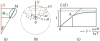
\includegraphics[scale=1]{figures/ch_07/fig_7_12.pdf}
		\caption[]{Explaining classical theory of paramagnetism: (a)---magnetic moment $\vec{M}$ and its projection $\vec{M}_H$ on magnetic field $\vec{H}$; (b)---calculating total magnetic moment of a paramagnetic; (c)---plot of the Langevin function.}
		\label{fig:7_12}
	\end{center}
	\vspace{-0.7cm}
\end{figure}

The probability for a dipole to align itself at an angle in the interval $(\theta, \theta+\deriv{\theta})$ to $\vec{H}$ [that is inside the solid angle $\deriv{\Omega}$; see \fig{7_12}(b)] is determined by the Boltzmann distribution function:
\begin{equation*}
    W = C_1\, e^{-\ab{U}{m}/\ab{k}{B}T}\, \deriv{\Omega} = C_1\, \exp\parenthesis{\frac{\mu_0 M H \cos\theta}{\ab{k}{B}T}}\, \deriv{\Omega}
\end{equation*}

\noindent
where $C_1$ is a normalization constant.

It may be seen from \fig{7_12}(b) that $\deriv{\Omega}=4\pi\sin\theta\,\deriv{\theta}$; therefore,
\begin{equation*}
    W = C_2\, \exp\parenthesis{\frac{\mu_0 M H \cos\theta}{\ab{k}{B}T}} \sin\theta\, \deriv{\theta}
\end{equation*}

\noindent
where $C_2$ is a new constant.

The average value of $M_H$ is
\begin{equation}\label{eq:7_46}
    \overline{M}_H = \overline{M\cos\theta} = M \frac{\displaystyle\int_0^\pi \cos\theta\,\exp\parenthesis{\dfrac{\mu_0 M H \cos\theta}{\ab{k}{B}T}} \sin\theta\, \deriv{\theta}}{\displaystyle\int_0^\pi \exp\parenthesis{\dfrac{\mu_0 M H \cos\theta}{\ab{k}{B}T}} \sin\theta\, \deriv{\theta}}.
\end{equation}

\noindent
If those integrals are evaluated, the result is
\begin{equation}\label{eq:7_47}
    \overline{M}_H = M \bracket{\parenthesis{ \frac{e^{\beta}+e^{-\beta}}{e^{\beta}-e^{-\beta}}} - \frac{1}{\beta}} = M \parenthesis{\coth\beta - \frac{1}{\beta}}
\end{equation}

\noindent
where
\begin{equation}\label{eq:7_48}
    \beta = \frac{M \mu_0 H}{\ab{k}{B}T}.
\end{equation}

The magnetization is
\begin{equation}\label{eq:7_49}
    \ab{J}{m} = n \overline{M}_H = n M \parenthesis{\coth\beta - \frac{1}{\beta}}
\end{equation}

\noindent
where $n$ is the number of atoms per unit volume, and the magnetic susceptibility is
\begin{equation}\label{eq:7_50}
    \chi = \frac{\ab{J}{m}}{H} = \frac{n M}{H}\parenthesis{\coth\beta - \frac{1}{\beta}}.
\end{equation}

Since the atomic dipoles acted upon by a field align themselves in its direction, such will be the direction of the magnetization of the body as a whole, which is characteristic of paramagnetics.

Let us expand $\coth\beta$ in a power series: $\coth\beta=\beta^{-1}+\beta/3-\beta^2/45+\ldots$. For $\beta\ll 1$, we can limit ourselves with the first two terms of the expansion. Then,
\begin{equation}\label{eq:7_51}
    \ab{J}{m} = \frac{n M \beta}{3} = \frac{nM^2}{3\ab{k}{B}T} \mu_0 H,\quad \chi = \frac{n\mu_0 M^2}{3\ab{k}{B}T}.
\end{equation}

In full agreement with experiment $\ab{J}{m}$ is directly proportional to $H$ and inversely proportional to $T$. The second of Eqs. \eqref{eq:7_51}, expresses the Curie law: $\chi=C/T$. The Curie constant $C=n\mu_0 M^2/(3\ab{k}{B})$.

For atoms $M\approx\ab{\mu}{B}$; then, for $H\approx\SI{e6}{\ampere\per\metre}$, we see that $MH\mu_0\approx\SI{e-23}{\joule}$ and for $T=\SI{300}{\kelvin}$, we see that $\ab{k}{B}T\approx\SI{3e-21}{\joule}$. Hence, the condition $\beta\ll 1$ is almost always satisfied.
Only in very strong fields and at very low temperatures is $\beta\gg 1$ and the direct proportionality between $\ab{J}{m}$ and $H$ is no longer maintained. In the limiting process, as $\beta\to\infty$, $\coth\beta\to 1$, and the magnetization becomes saturated, the corresponding maximum value being
\begin{equation}\label{eq:7_52}
    \ab{J}{s} = nM.
\end{equation}

\noindent
Magnetic saturation involves the alignment of magnetic moments of all atoms in the direction of the field.

The function $L(\beta)=\coth\beta-1/\beta$ is termed the \textit{Langevin junction}. Its plot is shown in \fig{7_12}(c). For small $\beta$'s, a good approximation for the plot is the segment of the straight line $0$A; as $\beta\to\infty$, the function $L(\beta)\to 1$.

\textbf{Fundamentals of quantum theory of paramagnetism.} The classical theory is incapable of providing a consistent explanation of the magnetic phenomena as the result of the motion of electric charges. The existence of molecular currents necessarily involves the acknowledgment of the fact of the stability of electronic motion in atoms, a fact unacceptable for classical physics. The assumption that all orientations of magnetic moments with respect to $H$ are possible, which is the basis of Langevin's classical theory, is also wrong. Those
difficulties have, on the whole, been overcome by the quantum theory of paramagnetism. Let's consider briefly the essence of this theory.

There are $2J+1$ ways in which the atomic magnetic moment $M_J$ may align itself in a magnetic field ($J$ is the intrinsic quantum number). The probability of each such orientation is determined
by the Boltzmann distribution $W=C\,e^{\mu_0M_{JH}H/\ab{k}{B}T}$ ($M_{JH}$ is the projection of $M_J$ on $H$). The average value of $M_{JH}$ will be
\begin{equation}\label{eq:7_53}
    \overline{M}_{JH} = \frac{\displaystyle\sum_{-J}^{+J} M_{JH} \exp\parenthesis{\dfrac{\mu_0 M_{JH} H}{\ab{k}{B} T}}}{\displaystyle\sum_{-J}^{+J} \exp\parenthesis{\dfrac{\mu_0 M_{JH} H}{\ab{k}{B} T}}}.
\end{equation}

The difference between \eqn{7_53} and the classical expression \eqref{eq:7_46} is that integration is replaced by summation over the discrete directions in which the vector $\vec{M}_J$ may be aligned. Evaluation of the sums in \eqn{7_53} yields the following result:
\begin{equation}\label{eq:7_54}
    \overline{M}_{JH} = g J \ab{\mu}{B} B_J(\beta)
\end{equation}

\noindent
where
\begin{align}
    \beta &= \frac{g J \ab{\mu}{B} H \mu_0}{2 \ab{k}{B} T}, \label{eq:7_55}\\
    B_J(\beta) &= \frac{2J+1}{2J} \coth\parenthesis{\frac{2J+1}{2J} \beta} - \frac{1}{2J} \coth\parenthesis{\frac{1}{2J}\beta}. \label{eq:7_56}
\end{align}

\noindent
Function $B_J(\beta)$ is termed the \textit{Brillouin function}.

The magnetization and the magnetic susceptibility are equal to
\begin{align}
    \ab{J}{m} &= n \overline{M}_{JH} = n g J \ab{\mu}{B} B_J(\beta), \label{eq:7_57}\\
    \chi &= \frac{n g J \ab{\mu}{B}}{H} B_J(\beta). \label{eq:7_58}
\end{align}

For $\beta\ll 1$, $B_J(\beta)\approx\beta(J+1)/(3J)$ and
\begin{equation}\label{eq:7_59}
    \ab{J}{m} = \frac{n g^2 \ab{\mu}{B}^2 J(J+1) \mu_0 H}{3 \ab{k}{B} T}, \quad \chi = \frac{n J (J+1) g^2 \ab{\mu}{B}^2 \mu_0}{3 \ab{k}{B} T}.
\end{equation}

It follows from \eqn{7_59} that for $\beta\ll 1$ the quantum theory results in a linear dependence of $\ab{J}{m}$ on $H$ and in an inverse dependence of $\ab{J}{m}$ and $\chi$ on $T$, which agrees with experiment. In strong fields and at very low temperatures $\beta\to\infty$,
\begin{equation*}
    \coth\parenthesis{\frac{2J+1}{2J} \beta} \to 1,\quad \coth\parenthesis{\frac{1}{2J}\beta} \to 1,\quad B_J(\beta) \to 1
\end{equation*}

\noindent
and the magnetization attains the saturation value
\begin{equation}\label{eq:7_60}
    \ab{J}{s} = n g J \ab{\mu}{B}.
\end{equation}

Materials used for experimental tests of the theory of paramagnetism are the solutions and crystalline hydrates of salts, which contain ions with nonzero magnetic moment. Such are, for instance, the ions of the elements of the groups of iron and rare earths. In solutions and in crystalline hydrates the ions are so far apart, that their interaction may be neglected, which is a necessary condition for paramagnetism. Experimental investigations of such compounds have produced results in good agreement with the theory.

\textbf{Paramagnetism of electron gas.} According to Eqs. \eqref{eq:7_51} and \eqref{eq:7_59}, paramagnetic susceptibility is inversely proportional to temperature. However, some metals have been discovered to exhibit paramagnetism independent of temperature. It was Wolfgang Pauli who demonstrated that this is due to the paramagnetism of free electrons that constitute the electron gas.

Figure \ref{fig:7_13}(a) shows the conduction band of a metal. It is schematically represented in the form of two half-bands containing electrons with opposite spin moments $\mu_s=\ab{\mu}{B}$. When $H=0$, the number of electrons in both half-bands is equal and the total magnetic moment of the electron gas is zero. When the field $H$ is applied, every electron of the left half-band acquires an additional energy $\ab{U}{m}'=-\mu_0\ab{\mu}{B}H$ and every electron of the right half-band an energy $\ab{U}{m}''=\mu_0\ab{\mu}{B}H$.
The result is the appearance of a difference between the quasi-Fermi levels $\ab{E}{F}''-\ab{E}{F}'=2\mu_0\ab{\mu}{B}H$ [\fig{7_13}(b)] for the electrons of the right and the left half-bands which is equalized by means of spin-flip of some of the electrons of the right half-band and their transition to the left half-band [\fig{7_13}(c)]. Since all the internal levels in the half-bands are occupied, the only electrons whose spins can be reversed are those occupying levels in the zone where the Fermi distribution is fuzzy [see \fig{5_6}(b)] and where there are vacant levels. The number of such electrons, according to \eqn{3_43}, is
\begin{equation}\label{eq:7_61}
    \Delta{n} \approx \frac{\ab{k}{B} T}{\ab{E}{F}} n
\end{equation}

\noindent
where $n$ is the electron gas concentration.

\begin{figure}[t]
	\begin{center}
		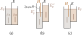
\includegraphics[scale=1]{figures/ch_07/fig_7_13.pdf}
		\caption[]{Calculating paramagnetism of free electrons.}
		\label{fig:7_13}
	\end{center}
	\vspace{-0.8cm}
\end{figure}

Of this number, $\Delta{n}'=C\,\exp\bracket{\mu_0\ab{\mu}{B}H/(\ab{k}{B}T)}$ electrons will have their magnetic moments oriented in the direction of $H$, and $\Delta{n}''=C\,\exp\bracket{-\mu_0\ab{\mu}{B}H/(\ab{k}{B}T)}$ against $H$ ($C$ is a constant). The magnetic moment per unit volume of a metal due to spin-flip is
\begin{equation*}
    \ab{J}{m$e$} = \parenthesis{\Delta{n}'-\Delta{n}''} \ab{\mu}{B} = C \ab{\mu}{B} \parenthesis{e^{\beta} - e^{-\beta}}
\end{equation*}

\noindent
where
\begin{equation*}
    \beta = \frac{\mu_0\ab{\mu}{B}H}{\ab{k}{B}T}.
\end{equation*}

Since $\Delta{n} =\Delta{n}'+\Delta{n}''=C\parenthesis{e^{\beta}+e^{-\beta}}$, it follows that $C=\Delta{n}\parenthesis{e^{\beta}+e^{-\beta}}^{-1}$. Substituting this into the expression for $\ab{J}{m$e$}$, we find
\begin{equation*}
    \ab{J}{m$e$} = \Delta{n} \ab{\mu}{B} \parenthesis{\frac{e^{\beta}-e^{-\beta}}{e^{\beta}+e^{-\beta}}} = \Delta{n} \ab{\mu}{B} \tanh\beta.
\end{equation*}

\noindent
For $\beta\ll 1$, $\tanh\beta\approx\beta$ and $\ab{J}{m$e$}=\Delta{n}\ab{\mu}{B}^2\mu_0 H/(\ab{k}{B}T)$. Substituting $\Delta{n}$ from \eqn{7_61}, we obtain
\begin{equation}\label{eq:7_62}
    \ab{J}{m$e$} \approx n \frac{\ab{\mu}{B}^2}{\ab{E}{F}} \mu_0 H.
\end{equation}

The paramagnetic susceptibility of the electron gas is
\begin{equation}\label{eq:7_63}
    \chi_e \approx n \frac{\mu_0 \ab{\mu}{B}^2}{\ab{E}{F}}.
\end{equation}

\noindent
A more accurate calculation yields
\begin{equation}\label{eq:7_64}
    \chi_e = \frac{3}{2} n \frac{\mu_0 \ab{\mu}{B}^2}{\ab{E}{F}}.
\end{equation}

It may be seen from \eqn{7_64} that the magnetic susceptibility of the electron gas should be independent of temperature, which is what is observed in practice.

\textbf{Production of low temperatures using the method of adiabatic demagnetization of paramagnetic samples.} The atoms of paramagnetic materials possess a permanent magnetic moment. In the absence of an external field, as a result of thermal motion of the atoms, the orientation of their magnetic moments is almost completely random. The quantitative measure of this disorder is the entropy $S$, which in this case is termed magnetic entropy $\ab{S}{M}$. In compliance with the Boltzmann principle
\begin{equation}\label{eq:7_65}
    \ab{S}{M} = \ab{k}{B} \ln{\ab{W}{M}}
\end{equation}

\noindent
where $\ab{W}{M}$ is the thermodynamic probability, which in this case, is equal to the number of ways the $n$ atoms of the paramagnetic sample can be distributed among the $2J+1$ sublevels into which every atomic level splits in a magnetic field. Its value may be obtained from the expression
\begin{equation}\label{eq:7_66}
    \ab{W}{M} = (2J + 1)^n.
\end{equation}

\noindent
Substituting \eqn{7_66} into \eqref{eq:7_65} we obtain
\begin{equation}\label{eq:7_67}
    \ab{S}{M} = \ab{k}{B} n \ln{(2J + 1)}.
\end{equation}

When the magnetic field is applied and its intensity increased, an ever increasing number of magnetic moments is oriented in the direction of the field, the result being a reduction in the magnetic entropy. When the state of magnetic saturation is reached, the greatest possible order in the arrangement of magnetic moments is established and $\ab{S}{M}$ vanishes. Hence, the process of magnetization of a paramagnetic sample up to saturation is accompanied by the decrease in its entropy by the amount
\begin{equation}\label{eq:7_68}
    \Delta{S} = \ab{S}{M} = \ab{k}{B} n \ln{(2J + 1)}.
\end{equation}

\noindent
If the magnetization is performed at a constant temperature $T$, the decrease in $S$ by the amount $\Delta{S}$ results in the generation of an amount of heat equal to $\Delta{Q}=T\Delta{S}$. This heat is transmitted from the sample to the surroundings, usually to liquid helium. After equilibrium has been established, the helium is removed and the sample is left thermally insulated. In such conditions it is slowly adiabatically demagnetized with the result that its entropy again rises by $\Delta{S}$. The rise in entropy requires heat, which can be supplied only by the thermal vibrations of the lattice, since the sample is thermally insulated from the surroundings. Because of that, its temperature drops. Using this method it was possible to obtain temperatures below \SI{0.001}{\kelvin}. The possibility of obtaining still lower temperatures is limited mainly by the fact that already at $H=0$, the atomic energy levels are, to some extent, split into sublevels because of the interaction of the magnetic moments with each other and with the nucleus.

\section{Origin of ferromagnetism}\label{sec:68}

\textbf{Elementary carriers of ferromagnetism.} A magnetized body acquires a magnetic moment $M$ made up of regularly oriented atomic magnetic moments and an angular momentum $P$ made up of regularly oriented atomic angular momenta. According to \eqns{7_17}{7_26}, the ratio $M/P$ must be equal to $q/2m$ if the magnetization is due to orbital magnetic moments of the atoms, and to $q/m$ if it is due to spin moments.

The appearance of a magnetic moment in the course of magnetization was first established in experiments of A. Einstein and W. J. de Haas and became known as the \textit{Einstein-de Haas effect}. In those experiments, a small iron rod $1$ suspended on a thin elastic thread $2$ was placed inside a solenoid $3$ [\fig{7_14}(a)]. In the course of magnetization the rod turned and twisted the thread. The direction of rotation of the rod changed with the change in the direction of magnetization. The angle of rotation was measured with the aid of mirror $4$ fixed on the rod which reflected a beam of light on scale $5$. The experiment made it possible to determine $M$ and $P$ and to find the gyromagnetic ratio $\gamma=M/P$.

\begin{figure}[t]
	\begin{center}
		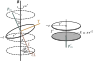
\includegraphics[scale=1]{figures/ch_07/fig_7_14.pdf}
		\caption[]{Experiments on the nature of ferromagnetism: (a)---the experiment of Einstein and de Haas; (b)---experiment of Barnett; (c,d)---experiment of Ioffe and Kapitza.}
		\label{fig:7_14}
	\end{center}
	\vspace{-0.8cm}
\end{figure}

S. J. Barnett made an experiment which was the reverse of the Einstein-de Haas experiment: he observed the magnetization of a quickly rotating iron rod. Such magnetization is caused by the tendency of electrons---thought of as tops possessing angular momenta---to arrange their axes of rotation (spins) in the direction of the rotation axis of the body [\fig{7_14}(b)]. In another experiment, the Soviet physicists A. F. Ioffe and P. L. Kapitza quickly heated a magnetized rod to a temperature above the Curie point. Before heating, the orientation of the ``electron tops'' was ordered [\fig{7_14}(c)] and their total angular momentum was nonzero. When heated to a temperature above the Curie point the ``tops'' changed their orientation to chaotic [\fig{7_14}(d)] and their total angular momentum became zero. Because of that, the demagnetized rod as a whole acquired a rotational momentum that could be measured in the experiment. Measuring in addition the magnetic moment of the magnetized rod one could find the gyromagnetic ratio $\gamma=M/P$.

The experiments demonstrated that the gyromagnetic ratio for ferromagnetic materials is $M/P=-q/m$, that is, equal to the gyromagnetic ratio for the intrinsic moments of the electron. This proved that ferromagnetism is due not to orbital but to spin magnetic moments of electrons, which is consistent with the electronic structure of the atoms of elements that exhibit ferromagnetism. Since the magnetic moments of closed shells are zero and since the outer valence electrons are collectivized in the process of formation of the metallic state, ferromagnetism must be a property solely of the transitional elements, which have incomplete inner shells. Those elements include the transitional metals of the iron group, which have an incomplete \enlevel{3}{d}{} shell, and rare earth elements with an incomplete \enlevel{4}{f}{} shell. Since, on the other hand, the orbital magnetic moments of the electrons of the \enlevel{3}{d}{} shell are ``frozen in'' and their contribution to the magnetic properties is negligible, ferromagnetism of the elements belonging to those groups can be due only to the atomic spin moments, which in this case are quite large (\tab{7_2}). This hypothesis was first expressed by the Russian scientist B. Rozing in 1892 and was exploited later by the French physicist Pierre Weiss. The latter assumed that there is an intense molecular field $H$ in a ferromagnetic proportional to the saturation magnetization $\ab{J}{s}$:
\begin{equation}\label{eq:7_69}
    H = \lambda \ab{J}{s}
\end{equation}

\noindent
where $\lambda$ is termed the \textit{molecular field constant}. This field is responsible for the spontaneous magnetization of a ferromagnetic.

The introduction of a molecular field made it possible to explain a wide range of phenomena observed in ferromagnetism. However, the nature of the field itself remained a mystery for a long time. At first, it was supposed that the origin of forces which orient the spin moments is purely magnetic, that they appear as a result of an ordinary interaction of spin magnetic moments (spin-spin interaction). The energy of this interaction is of the order of $\ab{U}{m}\approx\ab{\mu}{B}^2/a^2$, where $a$ is the interatomic distance in the lattice of the ferromagnetic. Substituting $\ab{\mu}{B}=\SI{9.27e-24}{\ampere\metre\squared}$ and $a\approx\SI{e-10}{\metre}$, we obtain $\ab{U}{m}\approx\SI{e-23}{\joule}$. This is about two orders of magnitude less than the room temperature thermal energy of a lattice atom which disturbs the orderly spin arrangement. It follows then that the magnetic spin interaction is incapable of effecting their parallel orientation, characteristic of the ferromagnetics, at temperatures below the Curie point, and that the origin of the molecular field, which effects such parallel spin orientation, should be nonmagnetic. Subsequently, this conclusion was proved by direct experiments of Ya. Dorfman.

\textbf{The role of exchange interaction in ferromagnetism.} In 1928, Frenkel made the assumption that the origin of the forces which are responsible for the definite mutual orientation of atomic magnetic moments is electrostatic. They are the result of exchange interaction of the electrons of inner incomplete atomic shells. We have already discussed this type of interaction in dealing with the nature of the covalent bond (see \sect{3}). The exchange interaction involves a change in the energy of the system. This is easily seen from the example of the simplest system of two hydrogen atoms (see \fig{1_5}). According to \eqns{1_11}{1_12} the energy of such a system is
\begin{equation}\label{eq:7_70}
    U = 2 E_0 + \parenthesis{\frac{K \pm A}{1 \pm S^2}}
\end{equation}

\noindent
where $E_0$ is the energy of two noninteracting hydrogen atoms, $K$ is the energy of Coulomb interaction of electric charges making up the atoms, $S$ is the overlap integral whose value lies in the range $0\ll S\ll 1$, and $A$ is the exchange energy (in Chapter \ref{chap:5} we called it the exchange integral).

Calculation shows that $A$ can be expressed by the following relation
\begin{equation}\label{eq:7_71}
    A = - J (\vecdotind{S}{i}{S}{j})
\end{equation}

\noindent
where $\vec{S}_i$ and $\vec{S}_j$ are the total spins of the interacting atoms, and $J$ is the exchange integral (it is a measure of the probability of electron $1$ going over to atom B and of electron $2$ going over to atom A). In the case of two interacting hydrogen atoms
\vspace{-10pt}
\begin{equation}\label{eq:7_72}
    J = \int \parenthesis{\frac{q^2}{r} + \frac{q^2}{r_{12}} - \frac{q^2}{\ab{r}{b$1$}} -\frac{q^2}{\ab{r}{a$2$}}} \ab{\psi}{a}(1) \ab{\psi}{b}(2) \ab{\psi}{a}(2) \ab{\psi}{b}(1)\, \deriv{V_1}\, \deriv{V_2}.
\end{equation}

\noindent
Here, $q^2/r$ and $q^2/r_{12}$ are the interaction energies of the nuclei between themselves and of the electrons between themselves, respectively; $-q^2/\ab{r}{b1}$ and $-q^2/\ab{r}{a2}$ are the energies of attraction of electron $1$ to nucleus b and of electron $2$ to nucleus a; $\ab{\psi}{a}(1)$ and $\ab{\psi}{b}(2)$ are the wave functions that describe the motion of electrons $1$ and $2$ around nuclei a and b, respectively; $\ab{\psi}{a}(2)$ and $\ab{\psi}{b}(1)$ are the wave functions that describe the probabilities for electrons $2$ and $1$ to be close to nuclei a and b, respectively, that is, the probabilities of the atoms A and B exchanging electrons; and $\deriv{V_1}$ and $\deriv{V_2}$ are volume elements.

It follows from \eqn{7_72} that both positive and negative terms enter the exchange integral. Therefore, the sign of the exchange integral may be either positive or negative. This is determined by the part played by the positive and negative terms of the exchange integral, which in its turn depends on the relation of the dimensions of the electron shells taking part in the formation of the exchange bond and on the interatomic distance.

The sign of the exchange integral determines what orientation of the spins of electrons taking part in the exchange bond is advantageous---the parallel or the antiparallel. It follows from \eqn{7_71} that
when the sign of the exchange integral is negative $(J<0)$, the exchange energy $A$ will be negative and, consequently, the system's energy $U$ will be less than the energy $2E_0$ of the individual atoms [see \eqn{7_70}] if the spins $\vec{S}_i$ and $\vec{S}_j$ of the electrons taking part in the exchange bond are antiparallel: $\vec{S}_i\downarrow\uparrow\vec{S}_j$. As has been mentioned in Chapter \ref{chap:1}, this case corresponds to the formation of a chemical bond between the atoms and the creation of a molecule [the symmetrical state described by \eqn{1_11}]; below we shall see that this is also a necessary condition for antiferromagnetism.

When the sign of the exchange integral is positive $(J>0)$, the exchange energy $A$ will be negative and the energy of the system as a whole will be less than the energy of the individual atoms if the spins $\vec{S}_i$ and $\vec{S}_j$ of the electrons taking part in the exchange bond are parallel: $\vec{S}_i\downarrow\downarrow\vec{S}_j$. Hence, the parallel orientation of the spins of neighbouring atoms may too be advantageous,, from the energy point of view, if their exchange integral is negative. This is the necessary condition for ferromagnetism since the parallel arrangement of spins and, consequently, of spin magnetic moments results in spontaneous magnetization, which is characteristic of ferromagnetics (see \fig{7_15}).

\begin{figure}[!t]
	\begin{minipage}[t]{0.47\linewidth}
		\begin{center}
            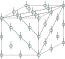
\includegraphics[scale=0.85]{figures/ch_07/fig_7_15.pdf}
    		\caption[]{Spontaneous magnetization of a ferromagnetic. Exchange forces cause parallel orientation of the spins of electrons belonging to inner partially filled shells.}
    		\label{fig:7_15}
		\end{center}
	\end{minipage}
	\hfill{ }%\hspace{-0.1cm}
	\begin{minipage}[t]{0.48\linewidth}
		\begin{center}
			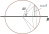
\includegraphics[scale=0.95]{figures/ch_07/fig_7_16.pdf}
			\caption[]{Dependence of exchange integral on the ratio of the lattice parameter to the diameter of the inner partially filled \enlevel{3}{d}{} shell in transition elements of the iron group.}
			\label{fig:7_16}
		\end{center}
	\end{minipage}
\vspace{-0.3cm}
\end{figure}

Figure \ref{fig:7_16} shows the dependence of the exchange integral $J$ on the ratio of the lattice constant $a$ to the diameter $d$ of the \enlevel{3}{d}{} shell of atoms of the iron group transition metals. It may be seen from \fig{7_16} that at $a/d>1.5$, the exchange integral is positive; at $a/d<1.5$ it turns negative, its absolute value increasing with the decrease in $a/d$. It follows then, that of all the transition metals only iron, cobalt, and nickel should be ferromagnetic, which is indeed the case. Manganese and other elements of the group, for which $a/d<1.5$, are not ferromagnetics. Should it, however, be possible to increase somewhat the lattice constant of manganese so that the ratio $a/d$ would approach $1.5$, one could expect manganese to become a ferromagnetic.

Experiments support this view. For instance, inclusion of small amounts of nitrogen into the manganese lattice increases its lattice parameter and results in the appearance of ferromagnetism. Ferromagnetic properties are also exhibited by the Mn-Cu-Al alloys (Heusler alloys) and by the compounds like \ce{MnSb} and \ce{MnBi} in which the distances between the manganese atoms are greater than in pure manganese crystals.

Hence, the necessary and adequate conditions for ferromagnetism are the existence of incomplete internal atomic shells and the positive sign of the exchange integral which cause the parallel orientation of the spins.

\textbf{Domain structure of ferromagnetic substances.} Let us isolate a region A inside a ferromagnetic crystal [\fig{7_17}(a)]. Suppose
that exchange forces establish a parallel orientation of spins of all the electrons of incomplete atomic shells, as shown in \fig{7_15}. Region A will be magnetized to saturation. What will be the equilibrium spin orientation in the region B below region A? If the spins in region B are oriented as in A, there are two magnets with like poles in contact with each other [\fig{7_17}(b)]. Such a state is unstable since it is characterized by the maximum energy of magnetic interaction. The stable state will be that in which the magnetic fields of the contacting regions are joined together, that is, a state in which the magnetization of the neighbouring regions of the crystal is opposite [\fig{7_17}(c)]. Calculations show that as long as the width of region A does not exceed several interatomic distances, the dominant factor is the first---the orientation action of the exchange forces---whose effect is to magnetize the layers of region B in contact with region A in the same direction as that of region A. As the area of A widens, the importance of the second factor (the increase in the energy of magnetic interaction) grows and finally it becomes predominant: the width of region A reaches a critical value and the magnetization of the neighbouring region B from now on proceeds in the opposite direction. The critical width of the region of spontaneous magnetization is dependent on many factors, but usually it does not exceed several micrometers.

\begin{figure}[t]
	\begin{center}
		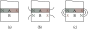
\includegraphics[scale=1]{figures/ch_07/fig_7_17.pdf}
		\caption[]{Ferromagnetic divided into domains (regions of spontaneous magnetization).}
		\label{fig:7_17}
	\end{center}
	\vspace{-0.8cm}
\end{figure}

Thus, in the absence of an external field a ferromagnetic crystal should consist of a great number of separate and rather small regions magnetized to saturation. Those regions have received the name of \textit{regions of spontaneous magnetization}, or \textit{domains}. Domains are separated by layers in which the orientation of the spins changes from that of one domain to that of the other (\fig{7_18}). Such transitional layers between domains became known as \textit{Bloch walls}. In iron, their thickness is about $300$ lattice constants (some \SI{1000}{\angstrom}). Figure \ref{fig:7_19} shows the domain pattern of a ferromagnetic predicted theoretically (a) and a photograph of the domain structure of an edge of a ferrosilicon crystal (b); arrows indicate the directions of spontaneous magnetization in the neighbouring domains.

\begin{figure}[t]
	\begin{center}
		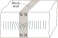
\includegraphics[scale=1]{figures/ch_07/fig_7_18.pdf}
		\caption[]{Structure of boundary layer separating two domains (``Bloch walls''); N denotes poles on the sample's surface.}
		\label{fig:7_18}
	\end{center}
	\vspace{-0.7cm}
\end{figure}

\begin{figure}[t]
	\begin{center}
		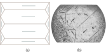
\includegraphics[scale=1]{figures/ch_07/fig_7_19.pdf}
		\caption[]{Domain structure of ferromagnetics: (a)---theoretically predicted pattern of a ferromagnetic's division into domains; (b)---photograph of an edge of ferrosilicon with decorated domain boundaries.}
		\label{fig:7_19}
	\end{center}
	\vspace{-0.8cm}
\end{figure}

\textbf{Qualitative analysis of the magnetization curve.} Spontaneous magnetization takes place in directions of easy magnetization. In the absence of an external field, the mutual orientation of the domains is such that the total magnetic moment of the ferromagnetic as a whole is zero [\fig{7_20}(a)], since this corresponds to the minimum of the system's free energy. When an external field $\vec{H}$ is applied, the ferromagnetic is magnetized acquiring a nonzero magnetic moment. The nature of the physical phenomena which take place during the magnetization of a ferromagnetic is such that the process may be subdivided into three stages.

\begin{figure}[t]
	\begin{center}
		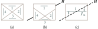
\includegraphics[scale=1]{figures/ch_07/fig_7_20.pdf}
		\caption[]{Processes involved in magnetization of a crystal: (a)---boundaries of four domains into which the crystal has been divided (the arrows indicate the direction of vector $\ab{\vec{J}}{m}$); (b)---displacement of boundaries and growth of the most favourably oriented domain $1$ with the increase in the magnetizing field $\vec{H}$; (c)---rotation of magnetization vector $\ab{\vec{J}}{m}$ in the direction of $\vec{H}$.}
		\label{fig:7_20}
	\end{center}
	\vspace{-0.7cm}
\end{figure}

\begin{figure}[t]
	\begin{center}
		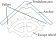
\includegraphics[scale=1]{figures/ch_07/fig_7_21.pdf}
		\caption[]{Magnetization plot of a ferromagnetic: $0$A---section corresponding to the process of displacement of domain boundaries, AB---section corresponding to rotation of magnetization vector, and BC---section corresponding to the paraprocess.}
		\label{fig:7_21}
	\end{center}
	\vspace{-0.8cm}
\end{figure}

\begin{enumerate}[(1)]
    \item \textit{Displacement of domain boundaries}. Place the crystal shown in \fig{7_20}(a) in a magnetic field $\vec{H}$. The orientation of the magnetization vector $\ab{\vec{J}}{m}$ of different domains with respect to $\vec{H}$ is not the same: $\ab{\vec{J}}{m}$ of the first domain makes the smallest angle with $\vec{H}$ and that of the third domain the largest. When $\vec{H}$ is increased it becomes advantageous from the viewpoint of energy for the most favourably oriented domain $1$ to grow at the expense of domains $2$, $3$, and $4$ [\fig{7_20}(b)]. The mechanism of this growth is the displacement     of the domain boundaries. For this reason, the first magnetization stage became known as the \textit{displacement process}.

    The displacement of the boundaries continues until the first domain spreads over the entire crystal. Figure \ref{fig:7_21} shows the magnetization curve of a single crystal. The displacement process is represented on this curve by the section $0$A. In small $\vec{H}$'s, magnetization proceeds smoothly and is reversible; in strong fields it is a jumpy and an irreversible process leading to the Barkhausen effect.

    \item \textit{Rotation}. When $\vec{H}$ is further increased, the spontaneous magnetization $\ab{\vec{J}}{m}$ begins to rotate towards the field [\fig{7_20}(c)]. The magnetization proceeds now at a much slower rate than in the first stage and ends when vector $\ab{\vec{J}}{m}$ coincides with $\vec{H}$. At this stage the magnetization reaches technical saturation (\fig{7_21}; section AB).

    \item \textit{Paraprocess}. After technical saturation is reached, the magnetization continues to grow with the increase in $\vec{H}$ although at a drastically reduced rate. The explanation is that, at any temperature other than absolute zero, not all the spins in the regions of spontaneous magnetization are oriented parallel to each other. Because of the thermal motion of atoms the orientation of some of the spins is antiparallel. The application of a strong magnetic field can effect the reorientation of these spins. The spin reorientation corresponding to the paraprocess is represented by the section BC.
\end{enumerate}

\section{Antiferromagnetism}\label{sec:69}

As was established in the preceding section, when the exchange integral is negative, the preferential orientation of the spins of neighbouring lattice sites is the antiparallel one. In this case, the spin arrangement can be also an ordered one, but there will be no spontaneous magnetization because the spin moments of the neighbouring lattice sites are antiparallel and compensate one another. Figure \ref{fig:7_22}(a) shows the magnetic structure of MnO determined with the aid of neutron spectroscopy (only the magnetically active Mn atoms are shown in the figure). The structure may be regarded as a complex one consisting of two sublattices magnetized in opposite directions. Such structure can exist only below a certain temperature termed the \textit{antiferromagnetic Curie point}, or the \textit{N\'eel point}.

\begin{figure}[t]
	\begin{center}
		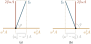
\includegraphics[scale=1]{figures/ch_07/fig_7_22.pdf}
		\caption[]{Magnetic structure of antiferromagnetic (a) and the temperature dependence of its magnetic susceptibility (b); the lattice of an antiferromagnetic (MnO) can be considered as consisting of two sublattices whose magnetic moments are antiparallel.}
		\label{fig:7_22}
	\end{center}
	\vspace{-0.8cm}
\end{figure}

At absolute zero, the magnetic moments of the sublattices are mutually compensated and the total magnetic moment of the antiferromagnetic is zero. As the temperature is raised, the antiparallel arrangement of the spins is gradually disturbed and the magnetization of the antiferromagnetic rises; it reaches its maximum at the N\'eel point, at which the orderly spin arrangement vanishes altogether, and the antiferromagnetic turns into a paramagnetic. As the temperature is raised still higher, the magnetization decreases in the same way as that of every paramagnetic. Figure \ref{fig:7_22}(b) shows the temperature dependence of the magnetic susceptibility of MnO whose N\'eel point is $\ab{T}{N}\approx\SI{120}{\kelvin}$ in a field $H\approx\SI{4e4}{\ampere\per\metre}$.

\section{Ferrimagnetism. Ferrites}\label{sec:70}

The magnetic moments of the sublattices in antiferromagnetics are equal in magnitude and opposite in direction with the result that they completely compensate one another. However, there are cases when the magnitude of the magnetic moments of the sublattices is not the same owing, for instance, to the difference in the number or in the nature of atoms that make up the sublattices [\fig{7_23}(a)]. This leads to the appearance of a finite difference in magnetic moments of the sublattices and to an appropriate spontaneous magnetization of the crystal. Such an uncompensated antiferromagnetism is termed \textit{ferrimagnetism}.

\begin{figure}[t]
	\begin{center}
		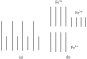
\includegraphics[scale=1]{figures/ch_07/fig_7_23.pdf}
		\caption[]{Schematic diagram of magnetic moments in a ferrimagnetic lattice in general (a) and specifically in magnetite $\ce{FeO}\cdot\ce{Fe2O3}$ (b). One of the sublattices is made up of the half of trivalent iron ions, the second sublattice being made up of the other half of trivalent iron ions and of bivalent ions of iron or of a substitute metal.}
		\label{fig:7_23}
	\end{center}
	\vspace{-0.8cm}
\end{figure}

The external behaviour of a ferrimagnetic is similar to that of a ferromagnetic, but because of the difference in their internal structure, the temperature dependence of their spontaneous magnetization may be quite different. For instance, the magnetization of a ferrimagnetic does not necessarily decrease monotonously with the rise in temperature but can pass through zero even before the N\'eel point is reached. Magnetite $\ce{FeO}\cdot\ce{Fe2O3}$ can serve as an example of a ferrimagnetic. The negative oxygen ions form a face-centered cubic lattice in which there are one bivalent ($\ce{Fe^2+}$) and two trivalent ($\ce{Fe^3+}$) iron ions to every $\ce{FeO}\cdot\ce{Fe2O3}$ molecule. The bivalent iron ions may be replaced by bivalent ions of other metals, for instance, Mg, Ni, Co, Mn, Cu, etc., so that the general formula of materials of this class known as \textit{ferrites}, assumes the form $\ce{MeO}\cdot\ce{Fe2O3}$, where Me stands for a bivalent metal. One of the sublattices of the complex ferrite lattice is made up of one half of the trivalent iron ions, and the other of the other
half of trivalent iron ions and of bivalent ions of iron or the substitute metal. The magnetic moments of the sublattices are antiparallel. Therefore, the magnetic moments of the trivalent iron ions are mutually compensated and the magnetization is due to the magnetic moments of the bivalent metal ions [\fig{7_23}(b)].

A remarkable property of ferrites is the combination of excellent magnetic parameters (high magnetic permeability, small coersive force, high saturation magnetization, etc.) with a high electrical resistance (of the order of \SI{e3}{\ohm\metre}). This particular property enabled ferrites to revolutionize the field of high and ultra-high frequency electronics. It is well known that ordinary low resistivity ($\approx\SI{e-3}{\ohm\metre}$) ferromagnetic materials cannot be used at such frequencies because of the extremely high eddy current losses. This was the reason why ferrites have occupied a unique position in this field.

Lately, ferrites with a high coersive force have been developed. They are used to construct permanent magnets capable of competing with electromagnets. Ferrites with a rectangular hysteresis loop are now widely used as digital storage elements in computers.

\section{Magnetic resonance}\label{sec:71}

The magnetic moment of atoms, ions, and radicals with unpaired electrons is determined by relation \eqref{eq:7_33}. There are $2J+1$ ways in which this moment may be aligned in a magnetic field $H_0$, there being correspondingly $2J+1$ different projections of the moment on the direction of the field. The energy corresponding to each such projection is
\begin{equation}\label{eq:7_73}
    \ab{U}{m} = \mu_0 M_{JH} H_0 = m_J g \mu_0 \ab{\mu}{B} H_0.
\end{equation}

\noindent
Therefore, an atomic energy level splits in a magnetic field into $2J+1$ sublevels (\fig{7_24}) the separations between which are
\begin{equation}\label{eq:7_74}
    \Delta{\ab{U}{m}} = g \mu_0 \ab{\mu}{B} H_0.
\end{equation}

\begin{figure}[t]
	\begin{center}
		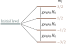
\includegraphics[scale=1]{figures/ch_07/fig_7_24.pdf}
		\caption[]{Splitting of a level of an atom with $J=3/2$ in a magnetic field.}
		\label{fig:7_24}
	\end{center}
	\vspace{-0.8cm}
\end{figure}

In the state of thermal equilibrium the atoms are distributed over those sublevels in accordance with the Boltzmann law:
\begin{equation*}
    n_1 = C\,\exp\parenthesis{-\frac{J g \mu_0 \ab{\mu}{B} H_0}{\ab{k}{B} T}},\quad n_2 = C\,\exp\bracket{-\frac{(J-1) g \mu_0 \ab{\mu}{B} H_0}{\ab{k}{B} T}},
\end{equation*}

\noindent
where $n_1$ is the number of atoms occupying the level with $m_J=J$, and $n_2$ the level with $m_J=J-1$.

To effect transitions of the atoms from the lower to the higher sublevels an external electromagnetic field can be used. Spectroscopic selection rules allow only of such transitions which result in a unit change in the magnetic quantum number:
\begin{equation}\label{eq:7_75}
    \Delta{m_J} = \pm 1
\end{equation}

\noindent
that is, only transitions between adjacent sublevels the energy difference between which is $g \mu_0 \ab{\mu}{B} H_0$. Such transitions can be excited by
an electromagnetic field whose energy quanta are
\begin{equation}\label{eq:7_76}
    \hslash\omega = g \mu_0 \ab{\mu}{B} H_0.
\end{equation}

Since transitions from the lower to the higher levels require a supply of energy, an intense absorption of electromagnetic energy will set in if condition \eqref{eq:7_76} is fulfilled.

Condition \eqref{eq:7_76} is the condition for \textit{electron paramagnetic resonance} (EPR). The resonance frequency, as implied by \eqref{eq:7_76}, is a function of the constant magnetic field intensity $H_0$. At $H_0\approx\SI{5.6e5}{\ampere\per\metre}$, $\ab{\nu}{res}\approx\SI{2e4}{\mega\hertz}$, which corresponds to the wavelength $\lambda\approx\SI{0.016}{\metre}$.

A similar phenomenon is the \textit{nuclear magnetic resonance} (NMR) due to the nuclear magnetic moment. For instance, in the case of protons, the nuclear resonance for $H_0\approx\SI{5.6e4}{\ampere\per\metre}$ occurs at a frequency of $\ab{\nu}{res}\approx\SI{30}{\mega\hertz}$, corresponding to a wavelength of electromagnetic radiation $\lambda\approx\SI{10}{\metre}$.

The first successful experiments on electron paramagnetic resonance were carried out by E. K. Zavoisky in 1944. He measured the losses of electromagnetic energy in an electrical circuit caused by paramagnetic absorption. In 1945 H. C. Torrey and R. V. Pound used Zavoisky's method for the first successful experiments on the nuclear resonance of protons in solid paraffin. That moment marked the start of a rapid development of microwave spectroscopy---a formidable branch of physics dealing with the interaction of radiowaves with matter.

The magnetic resonance is extremely widely used in different fields of science and technology.

The nuclear magnetic resonance is the main and the most accurate method for measuring the magnetic moments of atomic nuclei. NMR has been helpful in collecting the data on the structure of liquids, dielectric crystals, metals, semiconductors, and polymers. The first investigations of population inversion of energy levels utilized in lasers were carried out with its aid.

The electron paramagnetic resonance makes it possible to study particles possessing unpaired electrons and processes in which such particles take part. Those particles include the conduction electrons, the free and bonded radicals, many atoms and ions. EPR is successfully applied in the study of the mechanisms of chemical reactions, the radiation effects in matter and in live tissues, the electronic state of solids (metals, dielectrics, and semiconductors), and in many other important fields of science and technology.

\section{Fundamentals of quantum electronics}\label{sec:72}

\textbf{Stimulated radiation. ``Negative'' absolute temperatures.} The development of microwave spectroscopy in recent years, led to one of the most momentous technical discoveries---the discovery of the field \textit{quantum electronics}--- based on the ideas first put forward by Soviet physicists V. A. Fabrikant, N. G. Basov, and A. M. Prokhorov. Let us take a look at those ideas.

An external radiation directed at a quantum system causes not only the transitions from the lower to the upper levels, in which the energy is absorbed, but also the transitions from the higher to the lower levels, in which energy is liberated. Such radiation is termed \textit{stimulated}.

Consider the simplest quantum system with only two levels (\fig{7_25}). When $N$ radiation quanta pass through a system, the difference $\Delta$ in the number of transitions, from the lower levels to the higher levels and from the higher levels to the lower levels, will be proportional to the transition probability $w$ identical for both, the direct and the reverse processes, to the number of quanta $N$, and to the difference in the population of the levels $(n_2-n_1)$:
\begin{equation}\label{eq:7_77}
    \Delta = w N (n_2-n_1).
\end{equation}

\begin{figure}[t]
	\begin{center}
		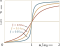
\includegraphics[scale=1]{figures/ch_07/fig_7_25.pdf}
		\caption[]{Two-level quantum system.}
		\label{fig:7_25}
	\end{center}
	\vspace{-0.8cm}
\end{figure}

In conditions of thermal equilibrium, the distribution of the particles over the levels is described by the Boltzmann law:
\begin{equation}\label{eq:7_78}
    n_1 = C\,e^{-E_1/\ab{k}{B}T},\quad n_2 = C\,e^{-E_2/\ab{k}{B}T},\quad,\quad \frac{n_2}{n_1} = \exp\bracket{-\frac{\parenthesis{E_2-E_1}}{\ab{k}{B}T}}.
\end{equation}

Since $E_2>E_1$, it follows that $n_2<n_1$, and because of that, resonance absorption exceeds stimulated radiation and the system absorbs incident electromagnetic energy eventually transforming it into heat.

For stimulated radiation to exceed resonance absorption, the thermal equilibrium of the system must be disrupted by raising the population of the higher levels above that of the lower levels, that is, to make $n_2>n_1$. Such population is termed \textit{population inversion}. Quantum states with population inversion may conveniently be described with the aid of the concept of negative absolute temperature. From \eqn{7_78} we have
\begin{equation}\label{eq:7_79}
    T = - \frac{\parenthesis{E_2-E_1}}{\ab{k}{B} \ln(n_2/n_1)}.
\end{equation}

In equilibrium, $n_2<n_1, E_2-E_1>0$, and $T>\SI{0}{\kelvin}$. In case of population inversion, $n_2>n_1, E_2-E_1>0$,, and consequently $T<\SI{0}{\kelvin}$. Figure \ref{fig:7_26} shows the occupancy of states at various temperatures.
At $T=\SI{0}{\kelvin}$, all the particles occupy the lowest level\footnote{To avoid contradiction with the Pauli exclusion principle, $E_1$ and $E_2$ must be taken to mean narrow energy bands: from $E_1$ to $E_1+\deriv{E}$ and from $E_2$ to $E_2+\deriv{E}$.} and the system's energy is at its minimum ($\ab{E}{min}=nE_1$). As the temperature rises, some of the particles go over to the higher level and the energy of the system increases.
At $T=\infty$, the population of the levels is equilized and the system's energy reaches the maximum value it can have in equilibrium [$\ab{E}{max}=n\parenthesis{E_1+E_2}/2$.
At $T<\SI{0}{\kelvin}$, the population of the higher level exceeds that of the lower level and, because of that, the energy of the systems turns out to be greater than $\ab{E}{max}$. Hence, the energy region corresponding to negative temperatures lies not below the absolute zero, as would appear at the first glance, but above infinite temperature. Should such a system be brought in contact with a body whose temperature
is positive, the heat would be transported from the system to the body until a state of thermal equilibrium would be reached.

\begin{figure}[t]
	\begin{center}
		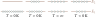
\includegraphics[scale=1]{figures/ch_07/fig_7_26.pdf}
		\caption[]{Level population at various temperatures.}
		\label{fig:7_26}
	\end{center}
	\vspace{-0.5cm}
\end{figure}

\begin{figure}[t]
	\begin{center}
		\includegraphics[scale=1]{figures/ch_07/fig_7_27.pdf}
		\caption[]{Population inversion in a two-level quantum system.}
		\label{fig:7_27}
	\end{center}
	\vspace{-0.8cm}
\end{figure}

It should be pointed out that negative temperature is a purely quantum effect and may be observed only in systems with a limited set of levels.

One may realize the population inversion in practice, for instance, by quickly reversing the direction of a constant magnetic field, so that the time of reversal would be less than the relaxation time. With the field $H_0$ in the initial direction the population of the lower level is greater than that of the upper one; when the field is reversed, quickly the initial population of the levels remains unchanged but with respect to the new field $H_0$ direction it will be populated inversely (\fig{7_27}).

\textbf{Principles of operation of masers.} Suppose that an external signal with the resonant frequency $\omega=(E_2-E_1)/\hslash$ is applied to a two-level system with a population inversion. This signal will induce the transitions of the particles: $E_2\to E_1$ and $E_1\to E_2$. Since in the case of population inversion the number of particles on the higher level exceeds that on the lower level, and since the transition probabilities
$w_{12}$ and $w_{21}$ are equal, the stimulated radiation $E_2\to E_1$ will exceed resonance absorption $E_1\to E_2$, and the signal will be amplified. Therefore, such a system will do the job of an amplifier of electromagnetic radiation. The term for it is \textit{paramagnetic amplifier} (usually \textit{maser}).

In practice, not two-level but three-level quantum systems are used for paramagnetic amplifiers. The active materials in them are diamagnetically diluted crystals of paramagnetic salts; in wide use are ruby crystals ($\ce{Al2O3}$) doped with chromium and germanium ions. Figure \ref{fig:7_28}(a) shows a quantum system with three levels: $E_1$, $E_2$, $E_3$. The dotted line represents the dependence of the number of particles $n$ on the energy $E$ in thermal equilibrium. Such a system
is placed in a magnetic field $H_0$ and irradiated with high-frequency electromagnetic radiation with a frequency $\omega_{13}=(E_3-E_1)/\hslash$. This process is termed \textit{pumping}. In pumping fields of high intensity [\fig{7_28}(b)], saturation is achieved, when the numbers of particles on the levels $E_1$ and $E_3$ are equal ($n_3=n_1$) and less than that on the level $E_2$: $n_1<n_2$, $n_3<n_2$. Should a signal with a frequency $\omega_{21}=(E_2-E_1)/\hslash$ be applied to such a system, it would be amplified by the stimulated transitions of the particles from the level $E_2$ to the level $E_1$. The system will work as an amplifier.

\begin{figure}[t]
	\begin{center}
		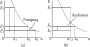
\includegraphics[scale=1]{figures/ch_07/fig_7_28.pdf}
		\caption[]{Excitation of paramagnetic amplifier (a) and radiation of amplified signal (b).}
		\label{fig:7_28}
	\end{center}
	\vspace{-0.8cm}
\end{figure}

For a high amplification factor the difference in the population of the levels must be as great as possible. The way to do it is to cool the system to liquid helium temperatures. The concentration of the
magnetic atoms should be low to exclude interaction of magnetic moments, which results in the widening of the absorption line and in the decrease in the amplification factor. One solution is to use diamagnetically diluted crystals of paramagnetic salts, of which the ruby crystal doped with chromium or germanium ions may serve as an example.
The main advantage of the paramagnetic microwave frequency amplifiers is their ability to work at very low temperatures and, consequently, at low noise levels. This makes it possible to receive signals too weak for amplifiers of conventional types. The frequency tuning of the amplifier is done by changing the intensity of the field $H_0$ which in its turn changes the resonance absorption frequency.

\textbf{Principles of operation of quantum generators.} To devise a laser on the basis of the negative temperature quantum system, a positive feedback should be provided to make sustained oscillations possible. To this end, the system is placed inside a cavity with reflecting walls. In conditions in which each spontaneously generated quantum $\hslash\omega$ stimulates the generation of, on the average, more than one quantum, the amplitude of the electromagnetic oscillations of the appropriate frequency $\omega$ will grow continuously. The system will become self-excited.
The radiative energy contained in the cavity is removed via a wave guide. Such cavities are termed \textit{cavity resonators}. They are constructed from highly conductive materials and their dimensions are close to the wavelength radiated by the laser. The feedback signal is provided by radiation reflected by the cavity walls, a careful choice of the dimensions and shape of the resonator being necessary to obtain the right phase relationship (the reflected radiation must be in phase with the generated one at the point of generation).

The first quantum generators were designed by N. G. Basov and A. M. Prokhorov. They used two-level oscillators and the generator operated on beams of ammonia molecules. The ammonia molecule $\ce{NH3}$ is made up of three hydrogen atoms arranged in the base of a triangular pyramid and a nitrogen atom in the pyramid's vertex [\fig{7_29}(a)]. This is the ground state of the molecule $E_1$. The molecule has an excited state $E_2$ [\fig{7_29}(b)] in which the nitrogen atom is forced into the base plane. The normal $\ce{NH3}$ molecule is asymmetric and by force of this has a nonzero dipole moment. The dipole moment of an excited molecule because of its symmetry is zero. This fact makes it possible to separate the normal and excited molecules by passing the molecular beam through a nonuniform
electric field. Such a field deflects normal polar molecules; the excited nonpolar molecules are not deflected.

\begin{figure}[t]
	\begin{center}
		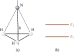
\includegraphics[scale=1]{figures/ch_07/fig_7_29.pdf}
		\caption[]{Ammonia molecule (a) and its energy levels (b).}
		\label{fig:7_29}
	\end{center}
	\vspace{-0.8cm}
\end{figure}

Figure \ref{fig:7_30}(a) represents a schematic view of a molecular generator. It is made up of three parts: the beam source A, the separation
system B, and the cavity resonator C.

The source of the molecular beam is a small space $1$ closed on one side by a fine mesh $2$. A gas pressure of one mmHg is maintained inside the space. The molecules forming the beam pass through the mesh into a vacuum chamber practically without collisions. A quadrupole condenser B [\fig{7_30}(b)] is placed in the way of the beam setting up a nonuniform field [\fig{7_30}(c)] that sorts out the molecules. The excited molecules (on the higher level) are concentrated close to the condenser axis and the normal molecules are deflected to the walls. In this way, the beam close to the condenser axis is made to contain mainly the excited molecules and thus a quantum system with population inversion, or with negative temperature, is created.

\begin{figure}[t]
	\begin{center}
		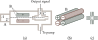
\includegraphics[scale=1]{figures/ch_07/fig_7_30.pdf}
		\caption[]{Schematic representation of a quantum generator operating on a beam of ammonia molecules: (a)---lay-out of amplifier (A is the source of beam of ammonia molecules, B the separation system, C the cavity resonator); (b)---quadrupole condenser of separating system; (c) electric field in condenser.}
		\label{fig:7_30}
	\end{center}
	\vspace{-0.8cm}
\end{figure}

From the separator B, the molecular beam enters the resonator C, turned to the frequency of the radiative transitions from the upper to the lower level [to the frequency $\omega=(E_2-E_1)/\hslash$] and induces in it electromagnetic oscillations with this frequency. The electromagnetic energy is transported via the wave guide $3$. The molecules in the beam practically do not interact and, because of that, the spectral line of the oscillations is very narrow (\SI{1}{\kilo\hertz} at $\nu=\SI{24}{\mega\hertz}$). Another advantage of the molecular generator is its long-term frequency
stability. The oscillation frequency is determined solely by the structure of the ammonia molecule (that is, by $E_2-E_1$) and is, therefore, independent of other generator circuit parameters. This made it possible to use the ammonia oscillator as a frequency standard. The error of a clock using such a frequency standard for its ``pendulum'' does not exceed one second in $300$ years of continuous
operation.

In recent years, quantum generators for the infrared and the optical spectral intervals (lasers) have been developed. Their use opens up wide possibilities for the development of communication, in locators, etc. For instance, an optical communication channel would be capable of carrying up to $10000$ TV programmes. Quantum generators nowadays are widely used for the machining of tough materials, in medicine, and in other fields of science and technology.
